\section{Background}

This section will explain the technical fundamentals which are necessary to understand the full bachelor thesis.

\subsection{The Scapy program}
\label{sec:scapy}

%UDS stack
\begin{wrapfigure}{r}{0.15\textwidth}
    %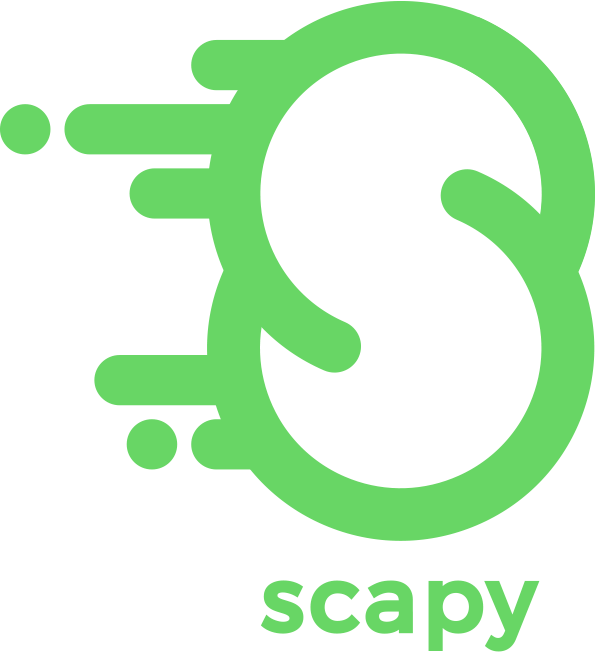
\includegraphics[width=0.1\textwidth]{scapy_logo}
    \raisebox{0pt}[\dimexpr\height-1.5\baselineskip\relax]{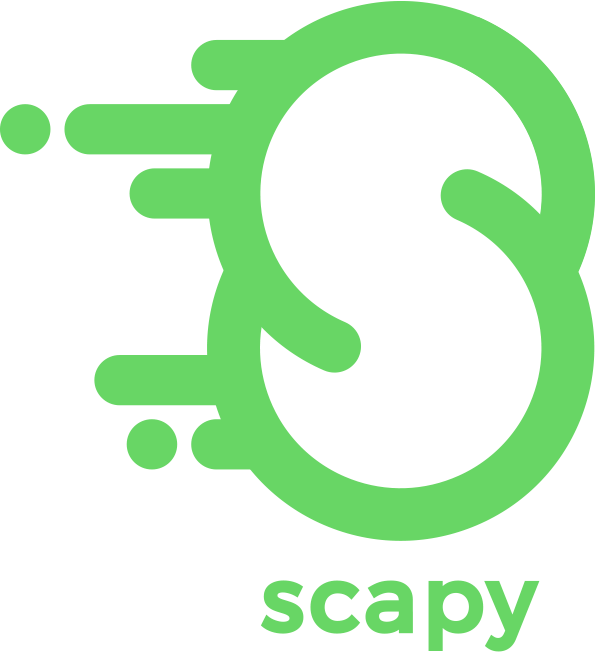
\includegraphics[width=0.15\textwidth]{scapy_logo}}
    %\label{fig:scapy-logo}
\end{wrapfigure}

The homepage of Scapy introduces itself with \cite{scapy}:
\begin{displayquote}
Scapy is a powerful interactive packet manipulation program. It is able to forge or decode packets of a wide number of protocols, send them on the wire, capture them, match requests and replies, and much more.
\end{displayquote}

So, it fulfills the requirements of protocol scanners:
\begin{itemize}
    \item Receiving and transmitting packets
    \item Support for many physical layers and transport protocols
    \item Simple definition of packet structures
    \item Matching requests with their responses
\end{itemize} 

It is used through a text-based user interface. This has the advantage of being lightweight, and working via ssh connections out-of-the-box. While being mainly a program, it can also be used as a library by importing the necessary classes and interfaces into the own Python program.

It supports Python 3 and also Python 2, even though its support has ended on 1st of January 2020. The following quote from a maintainer explains why \cite{scapy-py2}:

\begin{displayquote}
    Scapy is a tool that can be used in a very large number of situations. Often, you don't get to choose the Python interpreter you have when you run Scapy. So, [...] we need to keep supporting Python 2.7 as long as we can.
\end{displayquote}


\subsection{The CAN bus}

All communication performed and recorded in this paper with an ECU is done via the Control Area Network bus (CAN).

 Its specification is released in the ISO 11898. Each packet on this bus can transmit up to 8 bytes of payload and has an identifier which a length of either 11 or 29-bits, the former being more common. An identifier does not necessarily have to designate a physical device; it can also indicate one of several modules of a device.
 The maximum data rate is 1 Mbit/sec with a network length below 40 m. The higher the length, the lower the possible data rate, as can be seen in \autoref{tab:can-speed}.

\begin{table}[h]
    \centering
    \begin{tabular}{ccc}
    \hline
    \textbf{Bus Length (m)} & \textbf{Signaling Rate (Mbps)}\\
    \hline
    40 & 1 \\
    100 & 0.5 \\
    200 & 0.25 \\
    500 & 0.10 \\
    1000 & 0.05 \\
    \hline
\end{tabular}
\caption{Suggested Cable Length vs Signaling Rate \cite{slla270}.}
\label{tab:can-speed}
\end{table}

\subsubsection{Advantages for the automotive domain}

This bus is robust because it uses for the communication two wires  with differential signals. This means that if one wire is driven high, the other one is driven low. Thus, the receiver can reliably detect interferences by comparing these signals.

Moreover, CAN busses are using the bus network topology (see \autoref{fig:with-without-can}). This results in a smaller number of wires compared to star topologies, resulting in lower weight, which is an important factor for manufacturers.

%with-without-can
\begin{figure}[h]
    \centering
    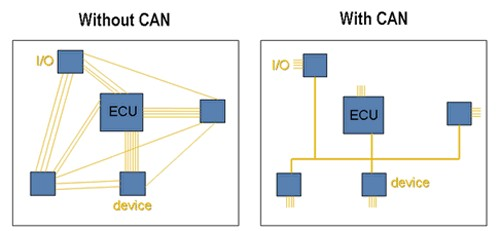
\includegraphics[width=0.7\textwidth]{with-without-can}
    \caption{CAN effect on decreasing the wire quantity \cite{Sharma2016}.}
    \label{fig:with-without-can}
\end{figure}

Last but not least, an important feature for the automotive application domain is the priority support. The lower the identifier, the higher the priority. Hence, if ECU1 and ECU2 transmit a CAN packet at exactly the same time, the packet with the lower identifier wins, the other one is discarded and will be retransmitted. This is called the Carrier Sense Multiple Access with Collision Detection (CSMA/CD) protocol \cite{Sharma2016}. For this reason, diagnostic CAN identifiers tend to have a high identifier \cite{Herrewegen2018}.

\subsubsection{Security vulnerabilities}

Thinking this one step further, CAN is vulnerable to denial of service attacks. This attack can be performed by flooding the CAN bus with zero-identifier messages resulting in drops of legitimate packets \cite{Buttigieg2017}.

Furthermore, Buttigieg et al. \cite{Buttigieg2017} describe three more security issues of the CAN bus protocol in their paper {Security Issues in Controller Area Networks in Automobiles}.
First, CAN packets do not contain any authentication information. An ECU receiving a message is not able to distinguish between a message from a legitimate ECU and a malicious one \cite{Buttigieg2017}. So, for example, if the state of an ECU is changed to a higher privileged state, all devices, including malicious ones, will have access to its newly unlocked services and information. Countermeasures exist in the form of performing authentication, but there is no satisfying solution yet, which fulfills cost-effectiveness, backward compatibility, support for vehicle repair and maintenance, sufficient implementation details, and acceptable overhead \cite{Bozdal2020}.
Also, originally, CAN bus networks lacked network segmentation, since each message is broadcasted and received by each node of the network \cite{Buttigieg2017}. Nowadays, car networks of higher-class cars like Audi and BMW are usually divided into less and more critical segments by so-called Gateway ECUs \cite{Bozdal2020}. Despite the increase in the level of security, this makes it more difficult to maintain the system, which is associated with increased costs \cite{Bozdal2020}.
The final security vulnerability is the lack of data encryption \cite{Buttigieg2017}. Lightweight encryption systems could be implemented, but are limited by the short length of the data field (8 bytes) and the limited computing power of ECUs \cite{Bozdal2020}.

Since all countermeasures described in the previous paragraph are limited, Intrusion Detection Systems (IDS) are emerging, with the advantages of not having to change the current CAN controller and not increasing bus traffic \cite{Bozdal2020}. Such a system has been implemented in the context of the PetS3 project \cite{spahn2018}.

\subsubsection{Using the can-utils}

Virtual CAN interfaces can be used for simulations or simple tests. They are supported natively by Linux without additional actions.
To create a virtual CAN interface, only one command in a Linux shell is required:
\begin{minted}{text}
sudo ip link add vcan0 type vcan
\end{minted}

The most common tool set to work with the CAN bus are the can-utils \cite{can-utils}, which can be usually installed with the package manager of the distributions. For example, the following command displays all messages of the CAN bus on interface \emph{vcan0}:
\begin{minted}{text}
candump vcan0
\end{minted}

Another important task is to send packets. This command sends a CAN packet with the identifier 0x123 and the payload \emph{01 02}:
\begin{minted}{text}
cansend vcan0 123#01.02
\end{minted}

Alternatively, Scapy can be used. There are two implementations of CAN sockets, namely a native one, which uses the native Linux kernel module, and a software-based one, which uses the Python-CAN package. The native implementation only supports Linux but is the preferred one because it uses the POSIX socket API from Linux and brings all its advantages, such as waiting for answers asynchronously without busy-waiting. However, Python-CAN has the advantage of also working on Windows and macOS.

An equivalent Scapy script which accomplishes the same as the just described \mintinline{text}{cansend} command, is:

\begin{samepage}
\begin{minted}{python}
from scapy.contrib.cansocket_native import CANSocket
from scapy.layers.can import CAN
socket = CANSocket("vcan0")
socket.send(CAN(identifier=0x123, data=b"\x01\x02"))
\end{minted}
\end{samepage}

\subsection{The ISO-TP transport protocol for CAN}

CAN packets have a payload size of 8 bytes. This is sufficient for most UDS requests, but not for many UDS responses. Thus, ISO-TP is used as the transport protocol on the CAN bus for UDS communication.

It is defined in ISO 15765-2 and increases the payload size from 8 bytes to 4095 bytes per message. At least one byte of each CAN packet is then transport protocol information, indicating whether this packet is a single frame or if it only contains a fragment of the actual payload.

\subsection{The UDS protocol}

UDS stands for \emph{Unified diagnostic services} and is an application protocol defined in ISO 14229. This protocol defines the structures of request and response packets for diagnostic purposes sent over an arbitrary data link \cite{iso14229}.

%UDS stack
\begin{figure}[h]
    \centering
    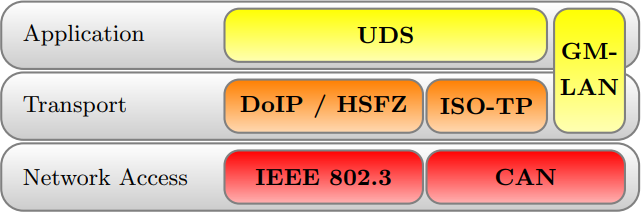
\includegraphics[width=0.7\textwidth]{uds-stack}
    \caption{The most common protocol stack for UDS \cite{Weiss2020}.}
    \label{fig:uds-stack}
\end{figure}

As shown in \autoref{fig:uds-stack}, the most common data links for the UDS protocol are the Ethernet and the CAN bus. Others can and are used as well, explicitly stated in the UDS standard are FlexRay, K-Line and LIN.

\subsubsection{Services}

The UDS protocol defines various services with different purposes.

The DiagnosticSessionControl (DSC) service with the identifier 0x10 is used to enable different diagnostic states in the ECU. All packets requesting this service specify this value as the first byte. The identifiers in the responses are defined as 0x40 added to the request identifier. Thus, for the DSC service the identifier of positive responses is 0x10 + 0x40 = 0x50. A negative response always has the identifier 0x7f.

Another example is the ReadDataByIdentifier (RDBI) service. Data records in an ECU are stored with an identifier as the key. This service allows to read these values from an external device. Since there may be data stored that should not be readable by everyone, there is another service called SecurityAccess (SA, 0x27) that allows to unlock the ECU for external devices.

The SA service uses the challenge–response authentication, in automotive terminology called seed-key protocol. The ECU sends a randomly generated value (the seed) to the client. Both devices generate a response (the key) based on the seed and the client sends its response to the ECU. If the keys match for the received and the generated response for the ECU, the client is authenticated \cite{iso14229}.

\begin{figure}[h]
    \centering
    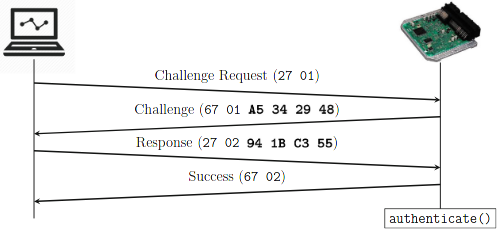
\includegraphics[width=0.7\textwidth]{key-seed}
    \caption{The challenge-response protocol \cite{Herrewegen2018}.}
    \label{fig:key-seed}
\end{figure}

\subsubsection{States}
\label{subsec:states}

There is always exactly one global UDS state active for an ECU. It influences the behavior of the ECU and can be changed by sending specific requests. Just a subset of services is able to accomplish this. For example, sending a request with the Security Access or the Diagnostic Session Control services to the ECU can affect its state. Whether the ECU has actually changed the state can be easily determined by checking whether the request has received a positive or negative response.

\begin{figure}[h]
    \centering
    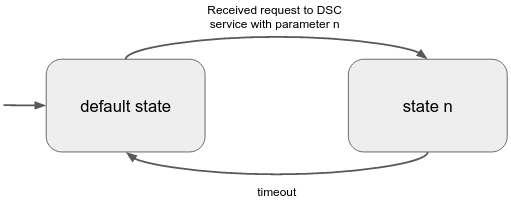
\includegraphics[width=0.7\textwidth]{ecu-state-behavior}
    \caption{State machine of ECUs for UDS.}
    \label{fig:ecu-state-behavior}
\end{figure}

The default state is the active state after the control unit is switched on. Without an external request, it remains in this state. \autoref{fig:ecu-state-behavior} illustrates the behavior of the ECU when a request is received for the DSC service and parameter value $n$. In the DSC service, each parameter value specifies a state. Thus, if the ECU designers integrated a state for $n$, the controller will respond positively. It will now remain in this state until there has been no UDS communication for usually five seconds, then it will automatically return to the default state. If the ECU designers did not integrate such a state, it will answer with a negative response and remain in the default state.


\subsection{The UDS Scanner}

The UDS Scanner was implemented in Scapy for the PetS3 project.

\subsubsection{Purpose}

\begin{figure}[h]
    \centering
    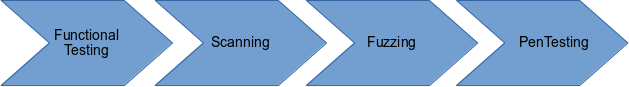
\includegraphics[width=0.8\textwidth]{automotive-security-testing-process}
    \caption{The Automotive Security Testing process.}
    \label{fig:automotive-security-testing-process}
\end{figure}

As \autoref{fig:automotive-security-testing-process} shows, the security testing process in the automotive domain contains a scanning step that aims to detect what services of a protocol are implemented and what information can be retrieved there \cite{Bayer2015}. The UDS Scanner fulfills these tasks. It can also be used for fuzzing and functional testing, even though scanning is its main use-case. The retrieved information assists for the manual PenTesting, the final step in this process.

\subsubsection{Procedure}

The UDS Scanner starts with scanning each service for the default state of the ECU (see \autoref{subsec:states}). While doing so, it detects new states, which will be scanned subsequently (for example with the DSC and SA service). So as long as new states are found during an iteration, the scan continues. After each iteration, the ECU is reset to return to the default state. From there, the next state to be scanned is activated through sending a sequence of UDS requests, representing an edge of a state machine. An ECU reset is usually done by switching off the ECU, waiting a few seconds, and switching it on again, although there is an ECUReset service in the UDS protocol. However, its specification states that the behavior is implementation-specific, so a power-based reset is the cleaner way.

The following pseudocode aims to make the procedure easier to understand:

\begin{samepage}
\begin{minted}{python}
class UDS_Scanner:
    def scan():
       states = [default_state]
       for state in states:
           ecu.reset()
           ecu.enter_state(state)
           for service in service_list:
               service.scan() # detects new states
       ecu.reset()
\end{minted}
\end{samepage}
